% Assignment 2 - Optimised Matrix Multiplication Approaches and Sparse Matrices
% Author: Tomas Santana
% Compile with pdflatex (Overleaf-ready).
% Every table and figure referenced here is auto-generated by
% assignment2/scripts/analyze_results.py and collect_system_info.py from
% the raw measurement CSVs.
\documentclass[11pt,a4paper]{article}

\usepackage[margin=2.5cm]{geometry}
\usepackage{amsmath,amssymb}
\usepackage{booktabs}
\usepackage{graphicx}
\usepackage{microtype}
\usepackage{caption}
\usepackage[hidelinks]{hyperref}

\graphicspath{{figures/}}

\title{\textbf{Optimised Matrix Multiplication Approaches}\\and Sparse Matrices\\
\large Assignment 2 --- Big Data, Grado en Ciencia e Ingeniería de Datos, ULPGC}
\author{Tomás Santana}
\date{Academic year 2026--2027}

\begin{document}
\maketitle

% =====================================================================
\begin{abstract}
\noindent This study answers two research questions about $n \times n$ matrix
multiplication under a strictly sequential, single-language (C) protocol.
\emph{Part A} asks how two classic optimisations---$i$-$k$-$j$ loop
reordering and cache blocking---change the runtime and memory profile of the
validated triple-loop baseline of Assignment 1 on identical inputs
($n \le 3000$, float64). \emph{Part B} asks under which tested sparsity
conditions a custom compressed-sparse-row (CSR) implementation of Gustavson's
sparse-by-sparse product beats the best dense kernel on identical logical
inputs (densities from $50\%$ down to $0.1\%$). Every configuration uses one
warm-up run, five measured repetitions, a monotonic kernel-only timer, a
per-run watchdog of 120\,s and a named peak-resident-memory metric; medians
and interquartile ranges (IQR) are reported and every raw measurement is
published. \emph{Main findings:} (i) both optimisations reduce kernel time at
large $n$ by up to a factor of several, with the gap widening as the working
set exceeds the last-level cache; (ii) the CSR product is orders of
magnitude faster than dense multiplication only at low density, and its
advantage collapses as fill-in densifies the product; (iii) the same
sparsity that saves time also inverts the memory advantage once the product
nnz approaches $n^2$. Conclusions are scoped to the tested hardware,
implementations and inputs.
\end{abstract}

% =====================================================================
\section{Introduction and Objective}

Matrix multiplication is the canonical $O(n^3)$ dense kernel and the
canonical case study for both \emph{locality-driven} optimisation and
\emph{sparse} representations. Assignment 1 established a validated,
reproducible triple-loop baseline in C (among other languages) and showed
its empirical growth on this machine. Assignment 2 extends that study along
two independent axes that the course specification requires to be discussed
separately: algorithmic/code optimisation of the dense kernel, and storage
format for sparse inputs.

\subsection*{Research questions}
\begin{enumerate}
    \item \textbf{RQ1 (Part A):} How do $i$-$k$-$j$ loop reordering and
    cache blocking affect the kernel time and peak memory of the validated
    $i$-$j$-$k$ baseline, for identical inputs, numeric type and timing
    boundary?
    \item \textbf{RQ2 (Part B):} For which tested density levels does a CSR
    (Gustavson) product outperform the best dense kernel on the \emph{same
    logical} sparse matrices, once conversion and output fill-in costs are
    accounted for?
\end{enumerate}

\subsection*{Hypotheses (declared before the measurements)}
\begin{itemize}
    \item H1: $i$-$k$-$j$ reordering will be faster than the baseline at
    moderate-to-large $n$ because the innermost loop streams rows of $B$
    and $C$ with unit stride; at small $n$ the difference will be small
    because everything fits in cache.
    \item H2: cache blocking will beat plain $i$-$k$-$j$ at large $n$ by
    reusing panels of $B$ inside the cache; the gain will depend on the
    block size and saturate once the panels no longer fit.
    \item H3: the CSR product will win by a large factor only at low
    density; the break-even density will decrease with $n$ because the
    product of two matrices with density $d$ has expected density
    $1-(1-d^2)^n$, which grows with $n$ (fill-in).
    \item H4: the peak resident memory of the sparse path will scale with
    $\mathrm{nnz}$ rather than with $n^2$, except that the CSR product
    stores the (possibly dense) output $C$ in sparse form, so at high
    density its storage exceeds the dense $3 \times 8n^2$ bytes.
\end{itemize}

% =====================================================================
\section{Background and References}

\subsection{Dense multiplication and data locality}
The straight-line triple loop computes
$C_{ij} = \sum_{k} A_{ik} B_{kj}$ in $\Theta(n^3)$ arithmetic work. The
loop \emph{order} does not change the operation count but changes which
elements are touched while they remain in cache. With the $i$-$j$-$k$ order
the innermost loop reads $A$ contiguously but $B$ column-wise (stride $n$),
which causes one cache miss per element on matrices larger than the cache;
with $i$-$k$-$j$ both $B$ and $C$ are streamed row-wise with unit stride
\cite{lam1991,goto2008}. Cache blocking (tiling) additionally partitions
the loops into panels so that working sets stay inside a chosen cache
level \cite{lam1991,goto2008,golub2013}. All dense kernels here perform
exactly the same floating-point work in the same accumulation order per
output element; only the traversal changes.

\subsection{Sparse storage and sparse-by-sparse products}
A CSR matrix stores $\texttt{rowptr}[0..n]$ (start offset of each row),
$\texttt{col}[\texttt{nnz}]$ (column index of each non-zero) and
$\texttt{val}[\texttt{nnz}]$ (its value), using
$4(n+1) + 12\,\texttt{nnz}$ bytes for float64 values \cite{davis2006,saad2003}.
Gustavson's algorithm multiplies two CSR matrices row by row: for row $i$
of $A$ it accumulates $A_{ik} B_{k,:}$ into a dense workspace indexed by
column, using a stamp array and a linked list so that clearing costs only
the touched columns; the finished row is sorted to obtain canonical CSR
\cite{gustavson1978}. The output of a product of two matrices with density
$d$ is not sparse in general: under an independent-Bernoulli model,
$\Pr[C_{ij} \neq 0] = 1 - (1-d^2)^n$, so for $nd^2 \gg 1$ the product is
essentially dense (\emph{fill-in}); this model is used below only as an
analytical reference, the measured $\texttt{nnz}_C$ is always reported
\cite{golub2013}.

\subsection{Floating-point determinism}
IEEE~754 addition is not associative \cite{ieee754}, so kernels that
traverse the operands in different orders (baseline vs.\ reordering) may
differ by small rounding amounts; tolerances are declared in
Section~\ref{sec:method}. The Gustavson kernel accumulates each output
element in a fixed $k$-order, which makes its results bit-comparable
across runs.

% =====================================================================
\section{Methodology}\label{sec:method}

\subsection{Implementations (custom student code in C)}
All kernels are custom C code (single file set under \texttt{src/c/}), share
one storage layout (contiguous row-major \texttt{double} arrays) and one
uniform contract: the kernel receives $A$, $B$ and a pre-allocated $C$ and
must produce $C = AB$ regardless of $C$'s previous contents; kernels that
accumulate zero $C$ \emph{inside} the timed region (an $O(n^2)$ cost against
$O(n^3)$ work), while allocation is always outside it. No value-dependent
shortcuts (skipping zeros) are allowed in the dense kernels, so arithmetic
work is identical for every dense method. The methods are:

\begin{itemize}
    \item \texttt{dense\_ijk\_baseline} --- the validated Assignment 1
    triple loop (same code, flags and layout); it assigns $C_{ij}$, so it
    needs no zeroing.
    \item \texttt{dense\_ikj\_reorder} --- optimisation 1: loop order
    $i$-$k$-$j$; the innermost loop streams rows of $B$ and $C$ with unit
    stride and is auto-vectorised by GCC.
    \item \texttt{dense\_blocked} --- optimisation 2: tiled $i$-$k$-$j$
    with block size $b$ (\texttt{g\_block\_size}). Table~\ref{tab:block-tuning}
    shows the tuning sweep; $b = 512$ is the default. For $n < b$ the
    kernel degenerates to plain $i$-$k$-$j$.
    \item \texttt{sparse\_csr\_gustavson} --- Part B: custom CSR
    structures plus Gustavson's row-wise SpGEMM with a dense accumulation
    workspace, stamp array and linked list; each output row is sorted by
    column index (canonical CSR). The $O(n)$ workspace and the geometric
    growth of the output arrays are allocated inside the timed kernel and
    freed before it returns (documented boundary).
    \item \texttt{dense\_to\_csr\_conversion} --- timed separately (never
    mixed into the kernel comparison): triplet gather + sort + scatter.
\end{itemize}

% Auto-generated by scripts/analyze_results.py -- do not edit.
\begin{table}[t]
\centering
\caption{Cache-block size tuning sweep: kernel time in ms (median of
the measured repetitions, 3 per sweep; $n=2000$ is covered by two
sweeps) for the blocked kernel. The default is
$b=512$.}
\label{tab:block-tuning}
\begin{tabular}{lccc}
\toprule
Block $b$ & $n=1500$ & $n=2000$ & $n=3000$ \\
\midrule
16 & 1305.5 & 3123.2 & -- \\
32 & 899.8 & 3854.8 & -- \\
64 & 2122.0 & 5198.7 & -- \\
128 & 1727.4 & 4314.0 & 13935.7 \\
256 & 1237.7 & 2433.0 & 7168.1 \\
512 (default) & -- & 2250.6 & 7652.9 \\
1024 & -- & 2266.5 & 7885.4 \\
\bottomrule
\end{tabular}
\end{table}


\subsection{Inputs}
\begin{itemize}
    \item \textbf{Part A:} the exact Assignment 1 matrices
    (\texttt{A\_n.csv}, \texttt{B\_n.csv}; float64, uniform in $[-10,10]$,
    Mersenne Twister seed~42), reused from \texttt{assignment1/data/matrices}.
    The bundled generator \texttt{scripts/generate\_matrices.py} reproduces
    them bit-identically, so the package is self-contained.
    \item \textbf{Part B:} generated deterministically inside the harness:
    each entry is exactly $0.0$ with probability $1-d$ and otherwise uniform
    in $[-10,10]$, drawn from a 32-bit LCG ($s \leftarrow 1103515245\,s +
    12345$) whose stream restarts from seed~42 for every configuration, so
    the zero patterns at a given $n$ are nested across densities. The dense
    and sparse paths consume the \emph{same} generated matrices.
\end{itemize}
Tested sizes: Part A $n \in \{10, 50, 100, 200, 400, 800, 1000, 1500, 2000,
3000\}$; Part B $n \in \{200, 500, 1000, 2000\}$ plus $n = 3000$ for
$d \in \{10\%, 1\%, 0.1\%\}$, with densities
$d \in \{50\%, 20\%, 10\%, 5\%, 1\%, 0.1\%\}$ (sparsity $= 100\%-d$).

\subsection{Environment}\label{sec:env}
% Auto-generated by scripts/collect_system_info.py -- do not edit.
\begin{table}[H]
\centering
\caption{Benchmarking machine and toolchain.}
\label{tab:env}
\begin{tabular}{ll}
\toprule
Component & Value \\
\midrule
CPU model & Intel(R) Core(TM) i7-14700HX \\
Physical cores / logical processors & 20 / 28 \\
Last-level cache (L3) & 33~MB \\
Total RAM & 31,7~GB \\
Operating system & Windows 10 (build 10.0.26300) \\
C compiler & gcc (Rev4, Built by MSYS2 project) 16.2.0 \\
Compile flags & \texttt{-O2 -march=native} (no OpenMP, 1 thread) \\
Analysis runtime & CPython 3.11.9 (pandas, matplotlib, numpy) \\
Timer & \texttt{clock\_gettime(CLOCK\_MONOTONIC)} (kernel only) \\
Memory metric & peak process working set (RSS), 5~ms sampling \\
\bottomrule
\end{tabular}
\end{table}


\subsection{Timing, repetitions and budgets}
The timer is \texttt{clock\_gettime(CLOCK\_MONOTONIC)} and measures the
\emph{kernel only}: input generation/loading and output allocation happen
outside the timed region; output initialisation happens inside it when the
kernel requires it (documented above). After every run the harness computes
$\mathrm{tr}(C)$ as an anti-dead-code-elimination checksum and stores it in
the CSV. Each configuration runs $1$ warm-up (kept in the CSV as
\texttt{repetition\_id = 0}, excluded from statistics) and $N = 5$ measured
repetitions; very small matrices ($n \le 50$) are multiplied in batches of
$100$ and the time is divided by the batch factor. A per-run watchdog of
$120$\,s aborts runs that exceed the declared budget; aborted runs are
recorded with \texttt{status = TIMEOUT} and \emph{no} execution time. The
memory metric is the \emph{peak process working set (resident set size)}
sampled every $5$\,ms by a background thread
(\texttt{GetProcessMemoryInfo}); as a sanity reference the analytic storage
of each representation is also reported (dense: $3\times 8n^2$ bytes;
sparse: CSR of $A$, $B$ and $C$ plus the $O(n)$ workspace). Sampled RSS and
analytic storage are different quantities and are never equated.

\textbf{Declared budgets.} Memory: 8\,GiB (largest configuration needs
$\approx 216$\,MiB of matrices; no OOM occurred). Time: $120$\,s per run.
The largest \emph{tested} size is $n = 3000$ for all Part A methods; the
largest \emph{attempted} size is $n = 4000$ with the baseline kernel
($\approx 294$\,s per run in Assignment 1), which is expected to hit the
watchdog and is reported as a TIMEOUT outcome in
Table~\ref{tab:dense-time}.

\subsection{Correctness}
The harness refuses to benchmark unless the correctness gate passes:
identity and zero matrices, a known $2\times2$ product, every dense kernel
against an independent $i$-$j$-$k$/$k$-$i$-$j$ reference at $n = 33, 64,
65$; CSR round-trip losslessness; Gustavson vs.\ dense product at four
densities; and sparse identity/zero products. Tolerances:
$\epsilon_{\text{abs}} = \epsilon_{\text{rel}} = 10^{-9}$ for these tests.
At benchmark scale the harness compares the full result matrices of all
executed methods (maximum absolute difference logged in
\texttt{crosscheck\_log\_*\_csv}); for $n \le 3000$ the worst-case
accumulation error $n\,\epsilon_{\text{mach}}\,|C|_{\max} < 10^{-6}$, so
cross-checks use $\epsilon_{\text{abs}} = 10^{-6}$. A dumped baseline
result is additionally verified against \texttt{numpy.matmul} by
\texttt{scripts/verify\_numpy.py} (NumPy is used only as a trusted
reference, never as a benchmarked method).

% =====================================================================
\section{Results}\label{sec:results}

All numbers below are computed by \texttt{scripts/analyze\_results.py} from
the raw CSVs in \texttt{data/results/}; every figure shows medians with
IQR-based variability. Table~\ref{tab:dense-time} and
Fig.~\ref{fig:dense-time} report the Part A kernel times,
Table~\ref{tab:dense-speedup} and Fig.~\ref{fig:dense-speedup} the
resulting speedups.

% Auto-generated by scripts/analyze_results.py -- do not edit.
\begin{table}[t]
\centering
\caption{Part A kernel execution time in ms (median [IQR] of the
measured repetitions; $N=5$; batch factor 100 applied for $n\leq50$).
\texttt{--} = no completed measurement: the baseline warm-up at
$n=3000$ exceeded the $120$\,s watchdog.}
\label{tab:dense-time}
\begin{tabular}{lccc}
\toprule
$n$ & Baseline i-j-k & Opt. i-k-j reorder & Opt. cache blocking \\
\midrule
10 & 0.00 [0.00] & 0.00 [0.00] & 0.00 [0.00] \\
50 & 0.03 [0.00] & 0.03 [0.00] & 0.03 [0.00] \\
100 & 0.29 [0.04] & 0.26 [0.01] & 0.27 [0.01] \\
200 & 2.56 [0.17] & 1.84 [0.09] & 1.90 [0.06] \\
400 & 24.03 [0.96] & 13.90 [0.29] & 15.32 [0.80] \\
800 & 320.70 [28.04] & 215.11 [25.86] & 207.44 [15.89] \\
1000 & 982.00 [6.16] & 434.39 [16.82] & 463.91 [11.29] \\
1500 & 4187.20 [58.79] & 1723.68 [43.76] & 1452.69 [99.09] \\
2000 & 31936.56 [1737.04] & 2960.28 [96.37] & 1764.16 [10.91] \\
3000 & -- & 21718.26 [484.08] & 11588.10 [92.55] \\
\bottomrule
\end{tabular}
\end{table}

\begin{figure}[t]
    \centering
    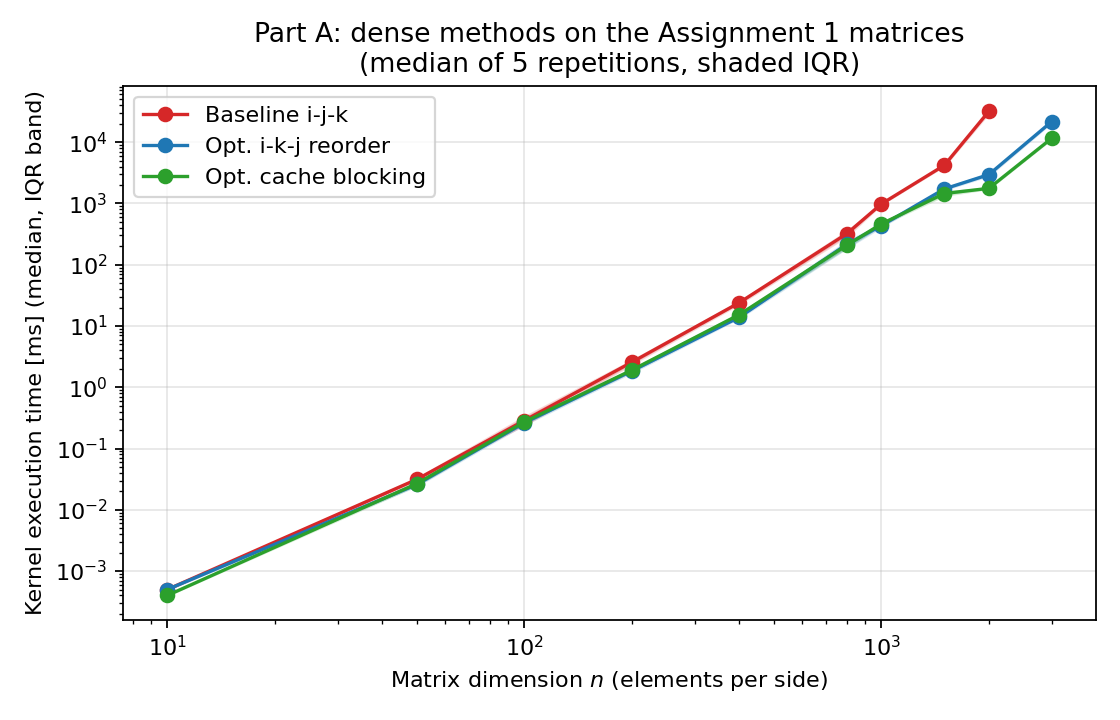
\includegraphics[width=0.92\textwidth]{fig_dense_time.png}
    \caption{Part A: kernel time vs.\ matrix dimension (log-log; median of
    5 repetitions; shaded band = IQR; batch factor 100 for $n \le 50$).}
    \label{fig:dense-time}
\end{figure}

% Auto-generated by scripts/analyze_results.py -- do not edit.
\begin{table}[t]
\centering
\caption{Speedup of the optimised dense methods over the validated
$i$-$j$-$k$ baseline (ratio of medians on identical inputs).}
\label{tab:dense-speedup}
\begin{tabular}{lcc}
\toprule
$n$ & $i$-$k$-$j$ reorder & Cache blocking \\
\midrule
10 & 1.00\times & 1.25\times \\
50 & 1.21\times & 1.18\times \\
100 & 1.09\times & 1.05\times \\
200 & 1.39\times & 1.35\times \\
400 & 1.73\times & 1.57\times \\
800 & 1.49\times & 1.55\times \\
1000 & 2.26\times & 2.12\times \\
1500 & 2.43\times & 2.88\times \\
2000 & 10.79\times & 18.10\times \\
\bottomrule
\end{tabular}
\end{table}

\begin{figure}[t]
    \centering
    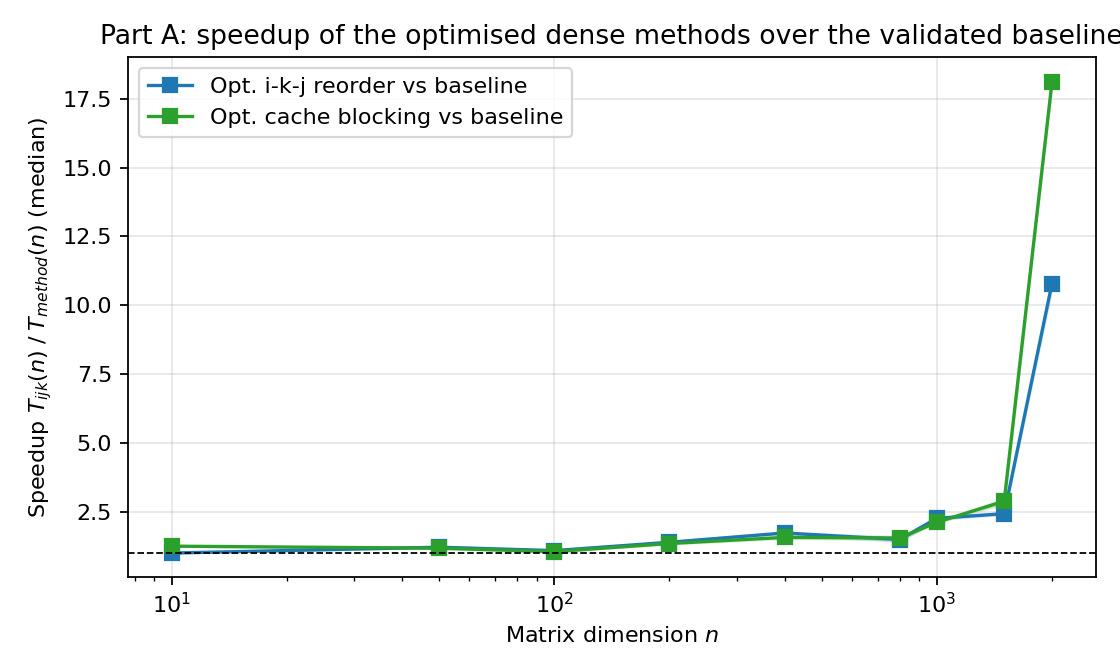
\includegraphics[width=0.9\textwidth]{fig_dense_speedup.png}
    \caption{Part A: speedup of the optimised kernels over the validated
    baseline (ratio of medians; shaded band from the IQR).}
    \label{fig:dense-speedup}
\end{figure}

\begin{figure}[t]
    \centering
    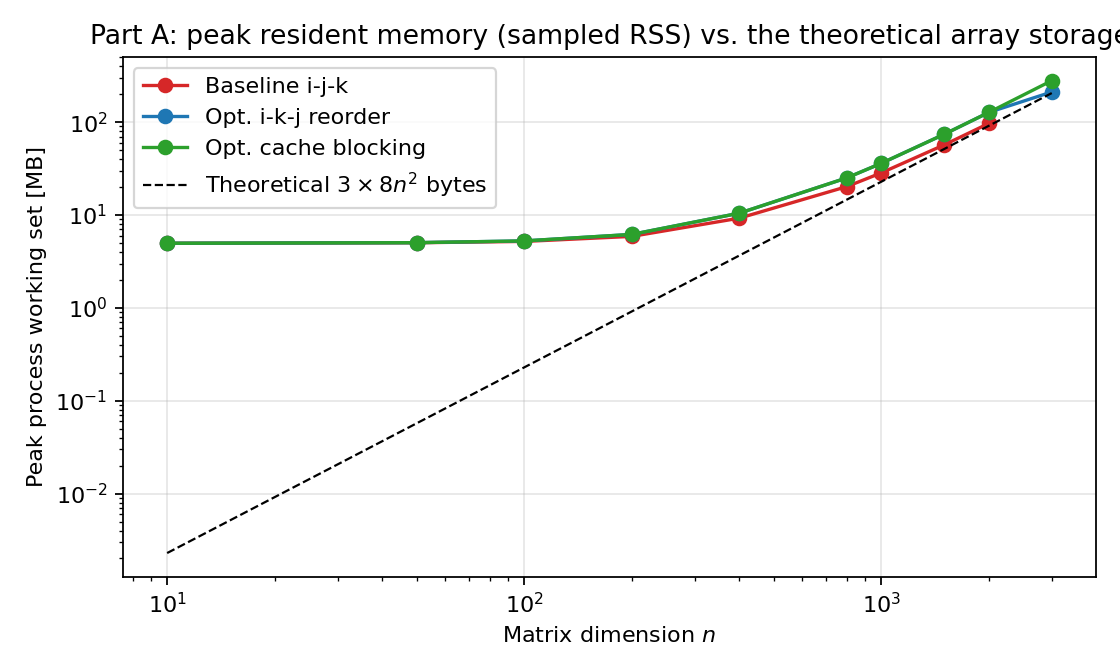
\includegraphics[width=0.9\textwidth]{fig_memory_dense.png}
    \caption{Part A: sampled peak resident memory vs.\ the analytic
    $3\times 8n^2$ array storage.}
    \label{fig:memory-dense}
\end{figure}

Part B is summarised in Table~\ref{tab:sparse-time} (times, speedup and
conversion cost), Table~\ref{tab:fill-in} with
Fig.~\ref{fig:fill-in} (output fill-in vs.\ the analytical model),
Table~\ref{tab:memory-partb} with Fig.~\ref{fig:memory-sparse} (memory),
and Figs.~\ref{fig:sparse-time}--\ref{fig:sparse-speedup} (time and
speedup vs.\ density).

% Auto-generated by scripts/analyze_results.py -- do not edit.
\begin{table}[t]
\centering
\caption{Part B: sparse CSR product (Gustavson) versus the best dense method (cache blocking) on identical logical inputs. Times are medians of $N=5$ repetitions in ms. `Speedup' is $T_{\mathrm{dense}}/T_{\mathrm{sparse}}$.}
\label{tab:sparse-time}
\resizebox{\textwidth}{!}{%
\begin{tabular}{rrcrrrrr}
\toprule
$n$ & Density [\%] & $nnz_A$ & $nnz_C$ & Dense [ms] & Sparse [ms] & Conv. [ms] & Speedup \\
\midrule
200 & 50 & 19\,883 & 40\,000 & 1.82 & 3.151 & 2.31 & $0.6\times$ \\
200 & 20 & 7\,844 & 39\,979 & 1.78 & 3.204 & 0.68 & $0.6\times$ \\
200 & 10 & 3\,986 & 34\,334 & 1.84 & 2.455 & 0.34 & $0.8\times$ \\
200 & 5 & 2\,063 & 15\,817 & 1.86 & 1.014 & 0.28 & $1.8\times$ \\
200 & 1 & 422 & 744 & 1.80 & 0.031 & 0.09 & $57.5\times$ \\
200 & 0.1 & 47 & 12 & 3.22 & 0.008 & 0.07 & $407.8\times$ \\
500 & 50 & 124\,730 & 250\,000 & 49.75 & 43.509 & 15.27 & $1.1\times$ \\
500 & 20 & 49\,748 & 250\,000 & 49.83 & 16.866 & 6.10 & $3.0\times$ \\
500 & 10 & 24\,953 & 248\,413 & 49.76 & 20.693 & 2.39 & $2.4\times$ \\
500 & 5 & 12\,498 & 179\,344 & 26.47 & 10.446 & 1.34 & $2.5\times$ \\
500 & 1 & 2\,520 & 12\,401 & 36.54 & 0.414 & 0.58 & $88.2\times$ \\
500 & 0.1 & 258 & 137 & 26.37 & 0.022 & 0.44 & $1198.5\times$ \\
1000 & 50 & 500\,287 & 1\,000\,000 & 428.32 & 285.474 & 67.90 & $1.5\times$ \\
1000 & 20 & 199\,732 & 1\,000\,000 & 426.29 & 103.029 & 27.58 & $4.1\times$ \\
1000 & 10 & 99\,841 & 999\,949 & 422.40 & 87.723 & 14.31 & $4.8\times$ \\
1000 & 5 & 50\,289 & 919\,343 & 423.73 & 82.684 & 8.27 & $5.1\times$ \\
1000 & 1 & 10\,068 & 95\,430 & 417.56 & 5.043 & 3.60 & $82.8\times$ \\
1000 & 0.1 & 1\,040 & 1\,094 & 418.91 & 0.057 & 2.01 & $7401.3\times$ \\
2000 & 50 & 2\,000\,233 & 4\,000\,000 & 3411.20 & 2199.435 & 300.59 & $1.6\times$ \\
2000 & 20 & 800\,262 & 4\,000\,000 & 3439.15 & 639.359 & 121.35 & $5.4\times$ \\
2000 & 10 & 399\,705 & 4\,000\,000 & 3442.70 & 429.638 & 62.37 & $8.0\times$ \\
2000 & 5 & 200\,400 & 3\,973\,788 & 3424.28 & 395.791 & 36.96 & $8.7\times$ \\
2000 & 1 & 39\,975 & 724\,865 & 3379.65 & 41.350 & 17.77 & $81.7\times$ \\
2000 & 0.1 & 4\,087 & 8\,322 & 3422.22 & 0.227 & 10.37 & $15056.0\times$ \\
3000 & 10 & 899\,426 & 9\,000\,000 & 11550.98 & 1165.146 & 147.40 & $9.9\times$ \\
3000 & 1 & 89\,797 & 2\,334\,617 & 11586.51 & 202.225 & 46.19 & $57.3\times$ \\
3000 & 0.1 & 9\,191 & 27\,375 & 11679.04 & 1.154 & 31.95 & $10121.4\times$ \\
\bottomrule
\end{tabular}}
\end{table}
\begin{figure}[t]
    \centering
    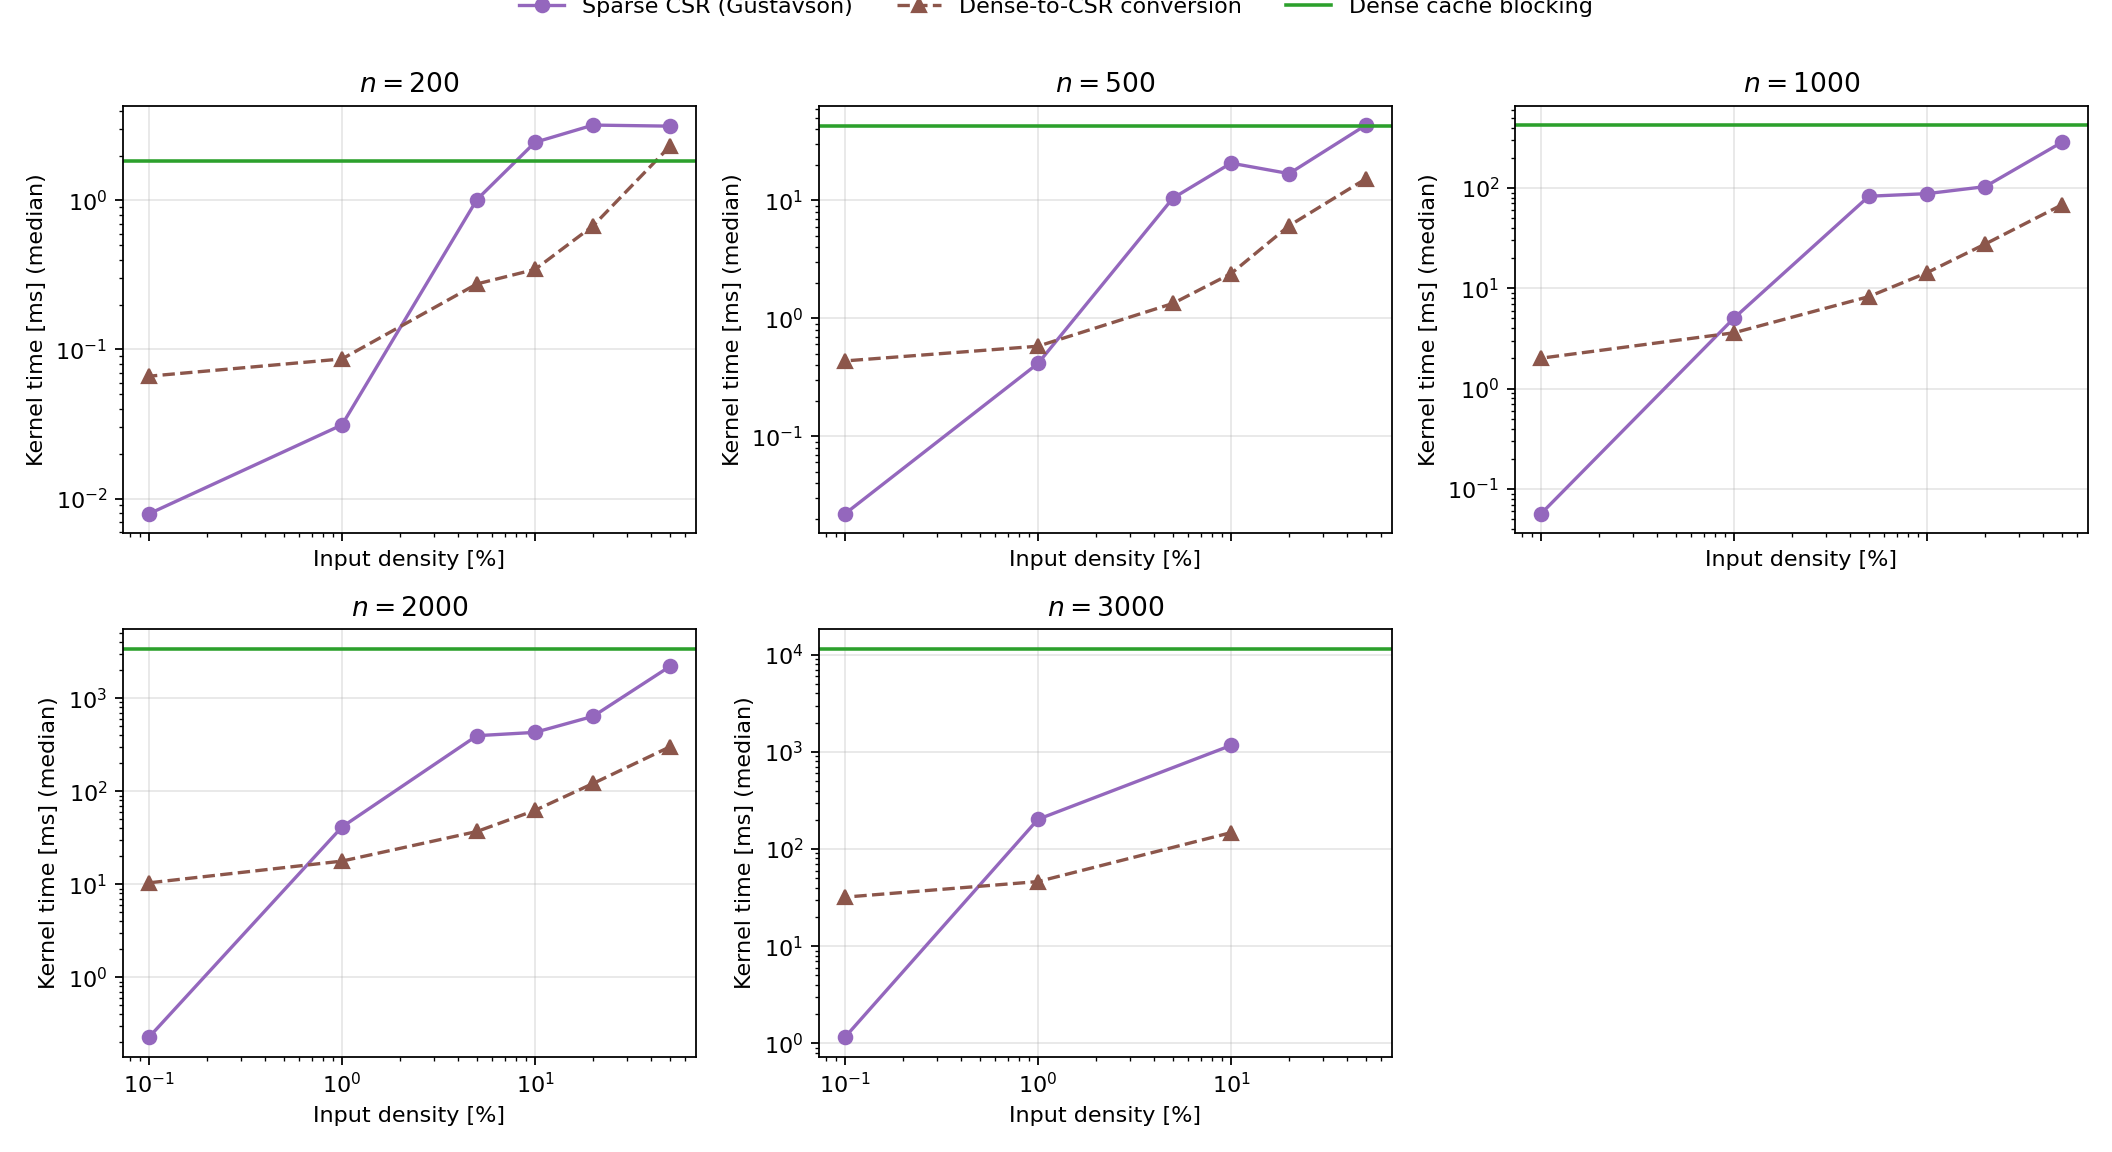
\includegraphics[width=\textwidth]{fig_sparse_time.png}
    \caption{Part B: kernel time vs.\ input density for the sparse product,
    the best dense kernel and the dense$\to$CSR conversion (median of 5
    repetitions; one panel per $n$).}
    \label{fig:sparse-time}
\end{figure}

\begin{figure}[t]
    \centering
    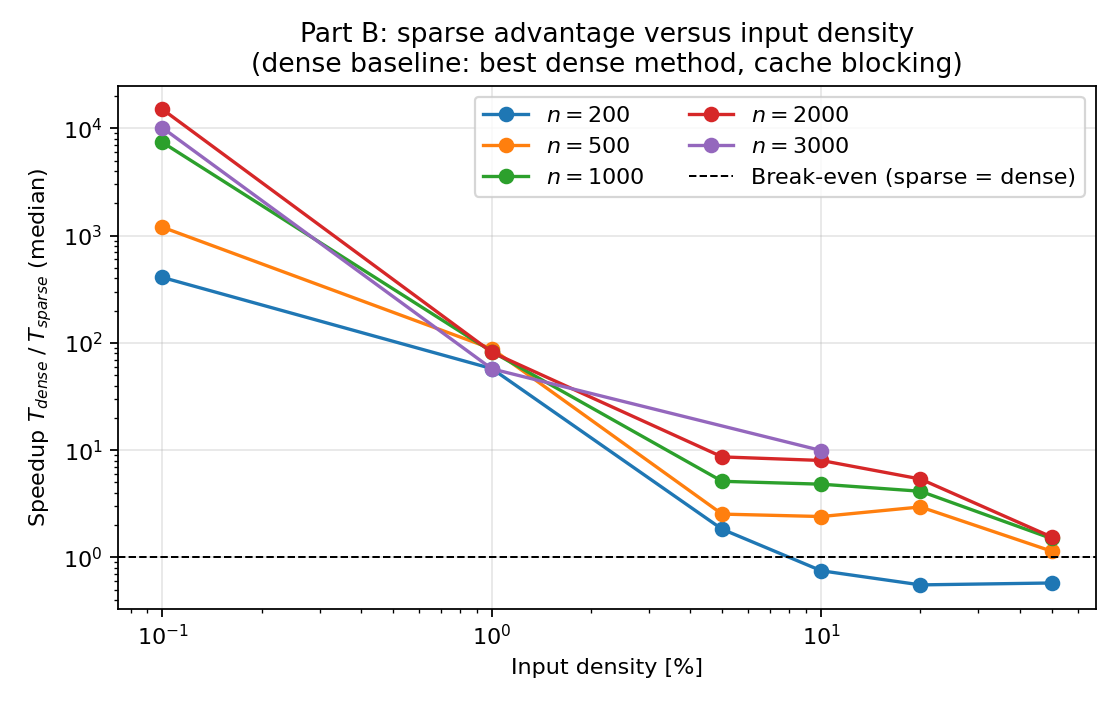
\includegraphics[width=0.9\textwidth]{fig_sparse_speedup.png}
    \caption{Part B: sparse advantage $T_{\text{dense}}/T_{\text{sparse}}$
    vs.\ input density (log-log; values above 1 favour the sparse path).}
    \label{fig:sparse-speedup}
\end{figure}

% Auto-generated by scripts/analyze_results.py -- do not edit.
\begin{table}[t]
\centering
\caption{Part B fill-in: measured output non-zeros versus the
independent-Bernoulli model $nnz_C \approx n^2\left[1-(1-d^2)^n\right]$.}
\label{tab:fill-in}
\begin{tabular}{rrrrr}
\toprule
$n$ & Density $d$ [\%] & $nnz_C$ measured & Model & Output density [\%] \\
\midrule
200 & 50 & 40\,000 & 40\,000 & 100.00 \\
200 & 20 & 39\,979 & 39\,989 & 99.95 \\
200 & 10 & 34\,334 & 34\,641 & 85.83 \\
200 & 5 & 15\,817 & 15\,754 & 39.54 \\
200 & 1 & 744 & 792 & 1.86 \\
200 & 0.1 & 12 & 8 & 0.03 \\
500 & 50 & 250\,000 & 250\,000 & 100.00 \\
500 & 20 & 250\,000 & 250\,000 & 100.00 \\
500 & 10 & 248\,413 & 248\,357 & 99.37 \\
500 & 5 & 179\,344 & 178\,486 & 71.74 \\
500 & 1 & 12\,401 & 12\,193 & 4.96 \\
500 & 0.1 & 137 & 125 & 0.05 \\
1000 & 50 & 1\,000\,000 & 1\,000\,000 & 100.00 \\
1000 & 20 & 1\,000\,000 & 1\,000\,000 & 100.00 \\
1000 & 10 & 999\,949 & 999\,957 & 99.99 \\
1000 & 5 & 919\,343 & 918\,172 & 91.93 \\
1000 & 1 & 95\,430 & 95\,167 & 9.54 \\
1000 & 0.1 & 1\,094 & 1\,000 & 0.11 \\
2000 & 50 & 4\,000\,000 & 4\,000\,000 & 100.00 \\
2000 & 20 & 4\,000\,000 & 4\,000\,000 & 100.00 \\
2000 & 10 & 4\,000\,000 & 4\,000\,000 & 100.00 \\
2000 & 5 & 3\,973\,788 & 3\,973\,216 & 99.34 \\
2000 & 1 & 724\,865 & 725\,110 & 18.12 \\
2000 & 0.1 & 8\,322 & 7\,992 & 0.21 \\
3000 & 10 & 9\,000\,000 & 9\,000\,000 & 100.00 \\
3000 & 1 & 2\,334\,617 & 2\,332\,736 & 25.94 \\
3000 & 0.1 & 27\,375 & 26\,960 & 0.30 \\
\bottomrule
\end{tabular}
\end{table}

\begin{figure}[t]
    \centering
    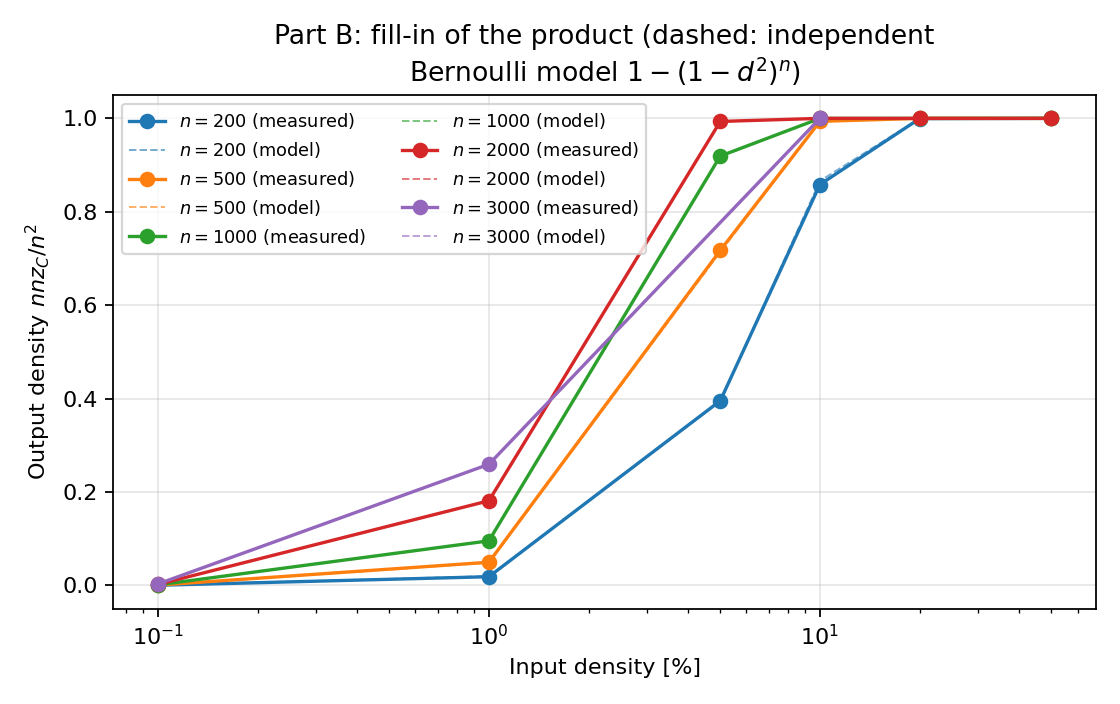
\includegraphics[width=0.9\textwidth]{fig_fill_in.png}
    \caption{Part B: measured output density $nnz_C/n^2$ vs.\ the
    independent-Bernoulli model $1-(1-d^2)^n$ (dashed).}
    \label{fig:fill-in}
\end{figure}

% Auto-generated by scripts/analyze_results.py -- do not edit.
\begin{table}[t]
\centering
\caption{Part B memory: sampled peak RSS of each kernel and theoretical
storage of the representations (dense: $3\times 8n^2$; sparse: CSR of
$A$, $B$ and $C$ plus the $O(n)$ Gustavson workspace).}
\label{tab:memory-partb}
\begin{tabular}{rrrrr}
\toprule
$n$ & Density [\%] & Peak RSS dense [MB] & Peak RSS sparse [MB] & Storage dense/sparse [MB] \\
\midrule
200 & 50 & 6.2 & 8.9 & 0.9 / 0.9 \\
200 & 20 & 6.7 & 9.2 & 0.9 / 0.6 \\
200 & 10 & 7.2 & 9.5 & 0.9 / 0.5 \\
200 & 5 & 7.7 & 8.9 & 0.9 / 0.2 \\
200 & 1 & 7.9 & 8.2 & 0.9 / 0.0 \\
200 & 0.1 & 7.9 & 8.2 & 0.9 / 0.0 \\
500 & 50 & 12.7 & 26.4 & 5.7 / 5.7 \\
500 & 20 & 15.9 & 27.6 & 5.7 / 4.0 \\
500 & 10 & 18.8 & 30.0 & 5.7 / 3.4 \\
500 & 5 & 21.7 & 30.2 & 5.7 / 2.4 \\
500 & 1 & 23.8 & 26.4 & 5.7 / 0.2 \\
500 & 0.1 & 24.5 & 26.4 & 5.7 / 0.0 \\
1000 & 50 & 41.7 & 94.8 & 22.9 / 22.9 \\
1000 & 20 & 54.1 & 99.4 & 22.9 / 16.1 \\
1000 & 10 & 64.1 & 108.6 & 22.9 / 13.8 \\
1000 & 5 & 75.7 & 116.2 & 22.9 / 11.7 \\
1000 & 1 & 86.2 & 98.8 & 22.9 / 1.4 \\
1000 & 0.1 & 87.4 & 95.1 & 22.9 / 0.1 \\
2000 & 50 & 156.1 & 369.9 & 91.6 / 91.6 \\
2000 & 20 & 201.9 & 388.3 & 91.6 / 64.2 \\
2000 & 10 & 247.8 & 425.0 & 91.6 / 55.0 \\
2000 & 5 & 293.6 & 465.3 & 91.6 / 50.1 \\
2000 & 1 & 339.1 & 395.6 & 91.6 / 9.3 \\
2000 & 0.1 & 347.4 & 378.6 & 91.6 / 0.3 \\
3000 & 10 & 462.5 & 860.5 & 206.0 / 123.7 \\
3000 & 1 & 565.2 & 716.3 & 206.0 / 28.9 \\
3000 & 0.1 & 591.9 & 663.0 & 206.0 / 0.7 \\
\bottomrule
\end{tabular}
\end{table}

\begin{figure}[t]
    \centering
    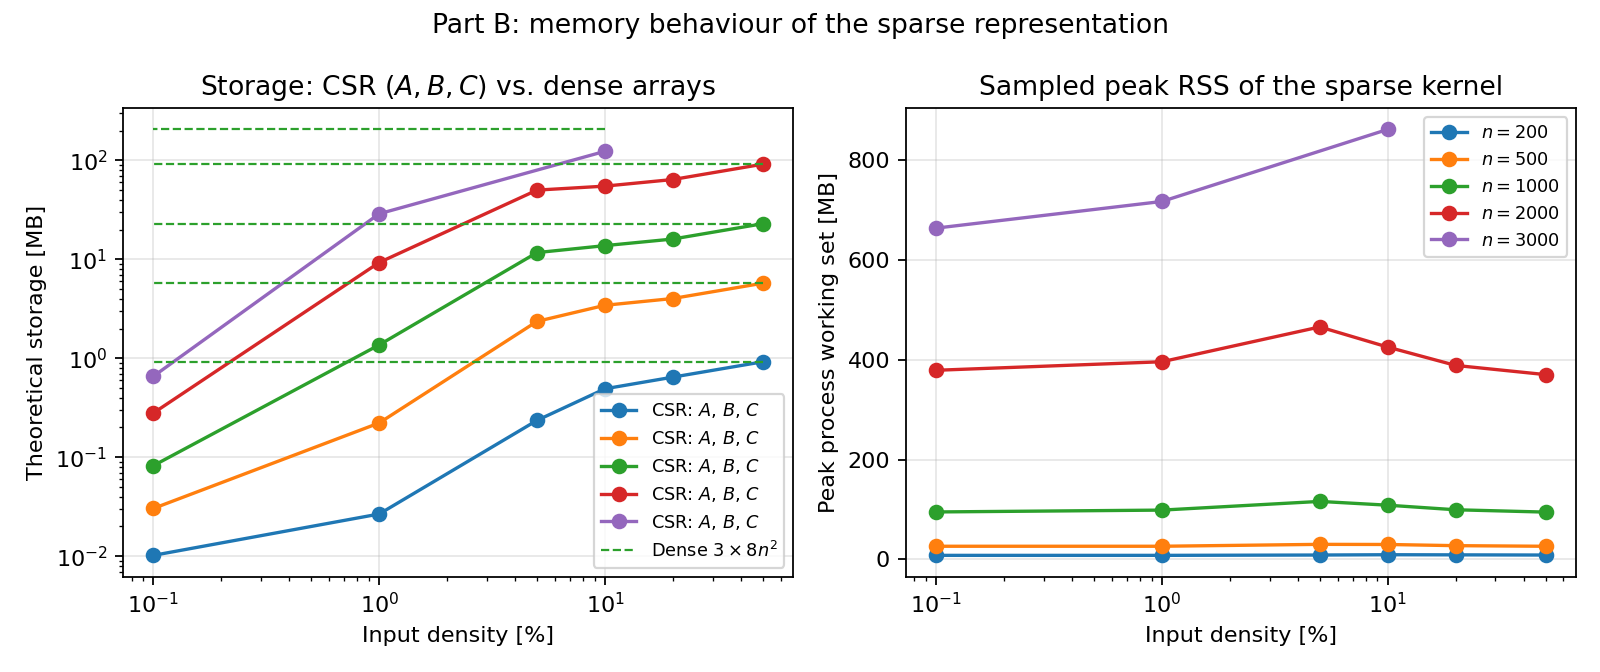
\includegraphics[width=\textwidth]{fig_memory_sparse.png}
    \caption{Part B memory: theoretical storage of the CSR path vs.\ the
    dense arrays (left) and sampled peak RSS of the sparse kernel (right).}
    \label{fig:memory-sparse}
\end{figure}

% =====================================================================
\section{Discussion}

% =====================================================================
\section{Conclusions}

% =====================================================================
\begin{thebibliography}{9}

\bibitem{horn2013}
R. A. Horn and C. R. Johnson, \emph{Matrix Analysis}, 2nd ed. Cambridge,
UK: Cambridge University Press, 2013.

\bibitem{gustavson1978}
F. G. Gustavson, ``Two algorithms for multiplying sparse matrices,''
\emph{BIT}, vol. 18, no. 4, pp. 425--434, 1978.

\bibitem{davis2006}
T. A. Davis, \emph{Direct Methods for Sparse Linear Systems}. Philadelphia,
PA, USA: SIAM, 2006.

\bibitem{saad2003}
Y. Saad, \emph{Iterative Methods for Sparse Linear Systems}, 2nd ed.
Philadelphia, PA, USA: SIAM, 2003.

\bibitem{lam1991}
M. E. Wolf and M. S. Lam, ``A data locality optimizing algorithm,'' in
\emph{Proc. ACM SIGPLAN Conf. Programming Language Design and Implementation
(PLDI)}, 1991, pp. 451--460.

\bibitem{goto2008}
K. Goto and R. A. van de Geijn, ``Anatomy of high-performance matrix
multiplication,'' \emph{ACM Trans. Math. Softw.}, vol. 34, no. 3, art. 12,
2008.

\bibitem{golub2013}
G. H. Golub and C. F. Van Loan, \emph{Matrix Computations}, 4th ed.
Baltimore, MD, USA: Johns Hopkins University Press, 2013.

\bibitem{ieee754}
IEEE Standard for Floating-Point Arithmetic, IEEE Std 754-2019.

\end{thebibliography}

% =====================================================================
\section*{References and Materials}

\subsection*{Repository structure}
\begin{verbatim}
assignment2/
├── src/c/            C kernels, CSR/Gustavson product, harness, validation
├── scripts/          generator, system info, NumPy cross-check, analysis
├── data/results/     raw measurements (CSV) + cross-check logs
├── report/           this report, generated figures and tables
└── README.md         build/run instructions and protocol
\end{verbatim}

\subsection*{Reproducibility}
Build and run commands, the CSV schema and the full experimental
configuration are documented in \texttt{assignment2/README.md}. The reused
Assignment 1 dataset can be regenerated bit-identically with
\texttt{scripts/generate\_matrices.py}; every raw measurement of this study
is published in \texttt{data/results/} and every table/figure is regenerated
deterministically by \texttt{scripts/analyze\_results.py}.

\subsection*{Generative AI disclosure statement}
The author used a large language-model assistant (the OpenCode coding agent,
powered by the MiMo LLM) for code scaffolding, experiment-planning
discussions, and language editing of this report. All implementations,
measurement protocols and analysis scripts were reviewed, compiled,
executed and validated by the author on the machine described in
Table~\ref{tab:env}; every reported number originates from the raw
measurement files included in this package. The author takes full
responsibility for the code, the data, the cited references and the
conclusions.

\end{document}
